\documentclass[11pt]{article}
\usepackage[utf8]{inputenc}
\usepackage[englisH]{babel}
\usepackage{bbm}
\usepackage{amssymb}
\usepackage{amsfonts}
\usepackage{amsmath}
\usepackage{chicago}
\usepackage[bottom]{footmisc}
\usepackage{setspace}
\usepackage[letterpaper]{geometry}
\usepackage{graphicx}
%\usepackage{subfigure}
\usepackage{adjustbox}
\usepackage{subcaption}
\usepackage{dcolumn}
\usepackage{floatrow}
\usepackage{epigraph}
\usepackage{environ}
\usepackage{minitoc}
\usepackage{comment}
%Includes "References" in the table of contents
\usepackage[nottoc]{tocbibind}
\usepackage{datatool}

%Import the natbib package and sets a bibliography style
%\usepackage[square,numbers]{natbib}
\usepackage{filecontents}
\usepackage{multibib}
\usepackage{natbib}
\bibliographystyle{apalike}
\newcites{supp}{ }

\usepackage[landscape]{geometry}
\usepackage{rotating}
\usepackage[T1]{fontenc}
\usepackage{tikz}
\usetikzlibrary{shapes,arrows}
\usepackage[final]{pdfpages}
%\usepackage[hyphenbreaks]{breakurl}
\usepackage{pdflscape}
\usepackage{pdfpages}
\usepackage[hyphens]{url}
\usepackage[hidelinks]{hyperref}
%\hypersetup{
%    urlcolor=blue,
%}
%\usepackage[colorlinks=true, linkcolor=maroon, urlcolor=maroon, citecolor=maroon]{hyperref}
\usepackage[numbered]{bookmark}
\usepackage{adjustbox}
\usepackage{booktabs}
\usepackage{qtree}
\usetikzlibrary{snakes} 
\usepackage{amsthm}
\theoremstyle{definition}  
\newtheorem{definition}{Definition}
\newtheorem{prop}{Proposition}
\newtheorem{assumption}{Assumption}
\urlstyle{same}
\usepackage{floatrow}
\floatsetup[table]{capposition=top}
\floatsetup[figure]{capposition=top}
\usepackage{graphicx}
\usepackage{caption}
\usepackage{geometry}
\usepackage[dvipsnames]{xcolor}
\usepackage{afterpage}
\usepackage{paralist}
\usepackage{colortbl}
\newcommand{\indep}{\rotatebox[origin=c]{90}{$\models$}}
\usepackage[table]{xcolor}
\usepackage{appendix}
\usepackage{placeins}
\def\subsectionautorefname{Section}
\def\subsectionautorefname{Section}
\def\appendixautorefname{Appendix}
%\newcommand*{\Appendixautorefname}{Appendix}
\usepackage{parskip}
\usepackage{multicol}
\usepackage{enumitem}

\usepackage{pgfplots}
\usepackage[T1]{fontenc}
\usepackage[utf8]{inputenc}

\usepackage{tgpagella}

\pgfmathdeclarefunction{gauss}{2}{%
  \pgfmathparse{1/(#2*sqrt(2*pi))*exp(-((x-#1)^2)/(2*#2^2))}%
}

\usepackage[toc,page,header]{appendix}

\usepackage{array}
\newcolumntype{L}[1]{>{\raggedright\let\newline\\\arraybackslash}p{#1}}

\setcounter{MaxMatrixCols}{30} 

\providecommand{\U}[1]{\protect\rule{.1in}{.1in}}


\newcolumntype{d}[0]{D{.}{.}{5}}

\geometry{verbose,tmargin=1in,bmargin=1in,lmargin=0.8in,rmargin=0.8in}


\doublespacing
\newcommand{\forceindent}{\leavevmode{\parindent=1em\indent}}
\makeatletter
%same as \subsection but level 4
\renewcommand\paragraph{\@startsection{paragraph}{4}{\z@}%
                                     {-3.25ex\@plus -1ex \@minus -.2ex}%
                                     {1.5ex \@plus .2ex}%
                                     {\normalfont\normalsize\bfseries}}
% number \paragraph
\setcounter{secnumdepth}{4}

\makeatother
%%%%%%%%%%%%%%%%%%%%%%%%%%%%%%%%%%%%%%%%%%%%%%%%%%%%%%%%%%%%%%
\begin{document}
\singlespacing

\noindent

\begin{center}
\LARGE{\textbf{Mock Monitoring Report for the Pre-Survey}}
\break
\break
\today
\normalsize
\end{center}
% \clearpage
\vspace{.8cm}

% \colorbox{yellow}{\textbf{Preview of Survey:} \href{https://harvard.az1.qualtrics.com/jfe/preview/previewId/1c54dd0d-b0c9-4176-ad48-0d399707c5df/SV_6hTTz50ZLuLrA9g?Q_CHL=preview&Q_SurveyVersionID=current}{Link}}
\vspace{.5cm}

\tableofcontents
\clearpage

This document reports summary statistics from the "Pre-Survey of Physicians." The survey was conducted on September 23, 2025, and targeted 250 primary care physicians and 250 specialists. On the first two days, we registered 5 completed responses. 

\clearpage

\section{Survey Deployment Tracking}

\begin{table}[H]
    \centering
    \caption{Survey Deployment Schedule: Initial and Reminder Emails}
    \begin{adjustbox}{width=1\linewidth} 
    \begin{tabular}{lccccccccccc} \toprule {Batch}&\shortstack{Specialty \\ type}&\shortstack{Number of \\ recipients}& \multicolumn{3}{c}{Initial email} & \multicolumn{3}{c}{Reminder email 1} & \multicolumn{3}{c}{Reminder email 2}  \\  \cmidrule(lr){4-6} \cmidrule(lr){7-9} \cmidrule(lr){10-12}  
    &  & &{Date}&{Day}&{Sent}&{Date}&{Day}&{Sent}&{Day}&{Date}&{Sent} \tabularnewline
\midrule \addlinespace[\belowrulesep]

1&PC&250&22sep2025 16:45:00&Monday&Yes&26sep2025 16:45:00&Friday&No&30sep2025 16:45:00&Tuesday&No \tabularnewline
1&SP&250&22sep2025 17:30:00&Monday&Yes&26sep2025 17:30:00&Friday&No&30sep2025 17:30:00&Tuesday&No \tabularnewline
2&PC&250&23sep2025 05:00:00&Tuesday&No&27sep2025 05:00:00&Saturday&No&01oct2025 05:00:00&Wednesday&No \tabularnewline
2&SP&250&23sep2025 05:00:00&Tuesday&No&27sep2025 05:00:00&Saturday&No&01oct2025 05:00:00&Wednesday&No \tabularnewline
2&ER&100&23sep2025 05:00:00&Tuesday&No&27sep2025 05:00:00&Saturday&No&01oct2025 05:00:00&Wednesday&No \tabularnewline
3&PC&250&24sep2025 05:00:00&Wednesday&No&28sep2025 05:00:00&Sunday&No&02oct2025 05:00:00&Thursday&No \tabularnewline
3&SP&250&24sep2025 05:00:00&Wednesday&No&28sep2025 05:00:00&Sunday&No&02oct2025 05:00:00&Thursday&No \tabularnewline
4&PC&250&25sep2025 17:00:00&Thursday&No&29sep2025 17:00:00&Monday&No&03oct2025 17:00:00&Friday&No \tabularnewline
4&SP&250&25sep2025 17:00:00&Thursday&No&29sep2025 17:00:00&Monday&No&03oct2025 17:00:00&Friday&No \tabularnewline
4&ER&100&25sep2025 17:00:00&Thursday&No&29sep2025 17:00:00&Monday&No&03oct2025 17:00:00&Friday&No \tabularnewline
\bottomrule 

    \end{tabular}
    \end{adjustbox}
    \label{tab:email_delivery}
          {\parbox{1\linewidth}{           %notes
		\scriptsize{{{ \textit{Notes:} A random sample of 1,000 primary care physicians, 1,000 specialists, and 200 emergency medicine physicians was assigned to different deployment schedules. The initial invitation and two reminder emails will be sent at varying dates and times according to this schedule. Assignment to schedules was randomized using uniform randomization.}}}}}
\end{table}

% \begin{table}[H]
%     \centering
%     \caption{Daily Tracking of Survey Responses}
%     \begin{adjustbox}{width=1\linewidth} 
%     \input{Pre-Survey/tables/initial_email_tracking_PC_SP_24sep2025_1015am_pt}
%     \end{adjustbox}
%     \label{tab:montly_kits}
%           {\parbox{1\linewidth}{           %notes
% 		\scriptsize{{{ \textit{Notes:} Counts are based on initial email recipients per batch. Email opened includes recipients who opened the email or started the survey; hard and soft bounces follow system status codes. Survey started includes any partial/expired attempts, and survey finished indicates completed surveys. All rates are calculated relative to batch recipients.}}}}}
% \end{table}

% \begin{table}[H]
%     \centering
%     \caption{Daily Tracking of Participant Compensation}
%     \begin{adjustbox}{width=0.75\linewidth} 
%     \input{Pre-Survey/tables/gift_card_tracking_PC_SP_24sep2025_1015am_pt}
%     \end{adjustbox}
%     \label{tab:email_delivery}
%           {\parbox{1\linewidth}{           %notes
% 		\scriptsize{{{ \textit{Notes:} Gift card distributions were processed through Tremendous. Counts are based on the number of recipients per batch. Compensation reflects the amount allocated per participant, with the total amount representing the full value disbursed for that batch. The updated balance reflects remaining funds after distribution.}}}}}
% \end{table}

\section{Completion Check}

%\input{completion_check_table.tex}
% tot participants, screend aout, innatentive, attrition, duration in  min (max, min and evr.)
%duplicated IP address

\begin{table}[H]
    \centering
    \caption{Survey Participation}
\begin{tabular}{lc}
\toprule
\textbf{Survey Completion}\\
 & Total \\
\hline
\textbf{Total \# of People Started Survey} & 2000 \\
\addlinespace
\textbf{Total Completion} & 374 \\
 & (0.19) \\
\textbf{Screened Out} & 1626 \\
 & (0.81) \\
\textbf{Attrition} & 0  \\
 & (0.00) \\
\hline
\end{tabular}

     \parbox{.9\linewidth}{
        	\vspace{.2cm}
        		\scriptsize{\scriptsize{{\emph{Notes}: The table provides an overview of survey participation. It outlines the initial survey participation numbers, including details on participants screened out, inattentive, and those who attrited.}}}}
    \label{tab:completioncheck}
\end{table}

\begin{figure}[H]
	\centering
	\caption{Histogram duration (in minutes)}
	\label{fig:hist_duration}
	\begin{adjustbox}{max width=\textwidth}
		\includegraphics{Pre-Survey/figures/hist_duration.pdf}
	\end{adjustbox}
	\parbox{.9\linewidth}{
		\vspace{.2cm}
		\scriptsize{\emph{Notes}: This figure displays a histogram depicting the duration (in minutes) that respondents took to complete the survey. I have omitted an outlier who took 7 hours and 18 minutes to complete the survey.}
	}
\end{figure}

\clearpage

\section{Screening}\label{demo}

\begin{table}[H]
    \centering
    \caption{Summary Statistics for Screeners}
    	\begin{adjustbox}{max width=0.8\textwidth}
\begin{tabular}{lc}
\toprule
\addlinespace
 & Total\\
\hline
\vspace{0.01em} \\ \emph{Medical degree} \\
\hspace{0.25cm} MD degree & 32\% \\
\hspace{0.25cm} DO degree & 33\% \\
\hspace{0.25cm} Other medical degree & 34\% \\
\hspace{0.25cm} No medical degree & 0\% \\
\vspace{0.01em} \\ \emph{Clinically active} \\
\hspace{0.25cm} Clinically active & 100\% \\
\hline
Observations & 347 \\
\bottomrule
\end{tabular}

\end{adjustbox}
     \parbox{.9\linewidth}{
        	\vspace{.2cm}
        		\scriptsize{\scriptsize{{\emph{Notes}: The table displays statistics for the overall sample of physicians. The numbers displayed are all shares.}}}}
    \label{tab:screen_table}
\end{table}

\clearpage

\section{Demographics}\label{demo}

\begin{table}[H]
    \centering
    \caption{Summary Statistics for Demographics}
              \begin{adjustbox}{width=0.55\linewidth}  
\begin{tabular}{l*{1}{cc}}
\toprule
                &Percentage (\%)&    Total\\
\midrule
\emph{Place of birth}&         &         \\
Born in U.S.    &       80&        5\\
\vspace{0.1em} \\ \emph{Age group}&         &         \\
Age <25         &        0&        5\\
Age 25–34       &       20&        5\\
Age 35–44       &       20&        5\\
Age 45–54       &       60&        5\\
Age 55–64       &        0&        5\\
Age 65+         &        0&        5\\
\vspace{0.1em} \\ \emph{Sex}&         &         \\
Male            &       40&        5\\
Female          &       60&        5\\
Other gender    &        0&        5\\
\vspace{0.1em} \\ \emph{Marital status}&         &         \\
Single          &        0&        5\\
Married         &      100&        5\\
Separated       &        0&        5\\
Widowed         &        0&        5\\
\vspace{0.1em} \\ \emph{Ethnicity}&         &         \\
Hispanic        &        0&        5\\
\vspace{0.1em} \\ \emph{Race}&         &         \\
White           &       60&        5\\
Black           &        0&        5\\
Native American &        0&        5\\
Pacific Islander&        0&        5\\
Asian           &       40&        5\\
Other race      &        0&        5\\
Mixed race      &        0&        5\\
\vspace{0.1em} \\ \emph{Political affiliation}&         &         \\
Republican      &       20&        5\\
Democrat        &       40&        5\\
Independent     &       40&        5\\
Other party     &        0&        5\\
Physician union at current workplace&       20&        5\\
Work ZIP (observed)&      100&        5\\
\bottomrule
\end{tabular}

\end{adjustbox}
     \parbox{.9\linewidth}{
        	\vspace{.2cm}
        		\scriptsize{\scriptsize{{\emph{Notes}: The table displays statistics for the overall sample of physicians. "Share (\%)" indicates the percentage of respondents in each group, and "Total" shows the number of observations used to calculate each percentage.}}}}
    \label{tab:demo_table}
\end{table}

\clearpage

\section{Categorization of Medical Fields by Physician Type} 


\begin{table}[H]
    \centering
    \caption{Categorization of Medical Field among Primary Care Physicians and among Specialists}
    \begin{adjustbox}{width=0.95\linewidth}  
    \begin{tabular}{lcccccc}\toprule
 & \multicolumn{3}{c}{Among Primary Care Physicians} & \multicolumn{3}{c}{Among Specialists} \\
\cmidrule(lr){2-4} \cmidrule(lr){5-7}
Medical field & \% PCP & \% Specialist & \% Difficult to classify & \% PCP & \% Specialist & \% Difficult to classify \\ \midrule
Family Medicine & 100 & 0 & 0 & 100 & 0 & 0 \\
Internal Medicine & 100 & 0 & 0 & 100 & 0 & 0 \\
Pediatrics & 100 & 0 & 0 & 100 & 0 & 0 \\
\midrule
Emergency Medicine & 0 & 50 & 50 & 0 & 33 & 67 \\
\midrule
Allergy and Immunology & 0 & 0 & 0 & 0 & 100 & 0 \\
Anesthesiology & 0 & 0 & 0 & 0 & 0 & 0 \\
Cardiology & 0 & 0 & 0 & 0 & 100 & 0 \\
Critical Care & 0 & 100 & 0 & 0 & 100 & 0 \\
Dermatology & 0 & 0 & 0 & 0 & 100 & 0 \\
Endocrine & 0 & 0 & 0 & 0 & 100 & 0 \\
Gastroenterology and Hepatology & 0 & 0 & 0 & 0 & 0 & 0 \\
General Surgery & 0 & 0 & 0 & 0 & 50 & 50 \\
Geriatrics & 100 & 0 & 0 & 50 & 50 & 0 \\
Hematology/Oncology & 0 & 0 & 0 & 0 & 100 & 0 \\
Infectious Disease & 0 & 0 & 0 & 0 & 0 & 0 \\
Nephrology & 0 & 100 & 0 & 0 & 0 & 0 \\
Neurology & 0 & 100 & 0 & 0 & 0 & 0 \\
Obstetrics and Gynecology & 0 & 0 & 0 & 0 & 100 & 0 \\
Ophthalmology & 0 & 100 & 0 & 0 & 100 & 0 \\
Orthopedic Surgery & 0 & 100 & 0 & 0 & 0 & 0 \\
Other medical field (e.g., Sleep Medicine, Sports Medicine, Medical Genetics) & 0 & 100 & 0 & 0 & 0 & 0 \\
Other surgical field (e.g., Neurosurgery, Plastic Surgery, ENT/Otolaryngology) & 0 & 0 & 0 & 0 & 100 & 0 \\
Pathology & 0 & 100 & 0 & 0 & 0 & 0 \\
Psychiatry & 0 & 0 & 0 & 0 & 0 & 0 \\
Pulmonology & 0 & 100 & 0 & 0 & 0 & 0 \\
Radiology & 0 & 100 & 0 & 0 & 100 & 0 \\
Rheumatology & 0 & 0 & 0 & 0 & 100 & 0 \\
Transplant & 0 & 0 & 0 & 0 & 0 & 0 \\
Urology & 0 & 100 & 0 & 0 & 100 & 0 \\
\bottomrule\end{tabular}

    \end{adjustbox}
    \label{tab:med_field_cat_phystype}
          {\parbox{1\linewidth}{           %notes
    		\scriptsize{{{ \textit{Notes:} The table displays statistics for the overall sample of physicians. Percentages (\%) indicates the percentage of respondents that select certain medical fields among a physician type. Percentages are calculated row-wise within each physician type, so values across columns for a given medical field sum to 100\% wihtin each physician type.}}}}}
\end{table}

\begin{table}[H]
    \centering
    \caption{Among Primary Care Physician: Categorization of Medical Field by Physician Type}
    \begin{adjustbox}{width=0.95\linewidth}    
    \begin{tabular}{lrrrrrrr}\toprule
 & \multicolumn{2}{c}{Primary Care Physician} & \multicolumn{2}{c}{Specialist} & \multicolumn{2}{c}{Difficult to classify} & \multicolumn{1}{c}{All groups} \\
\cmidrule(lr){2-3} \cmidrule(lr){4-5} \cmidrule(lr){6-7} \cmidrule(lr){8-8}
Medical field & Total & Percentage (\%) & Total & Percentage (\%) & Total & Percentage (\%) & Percentage (\%) \\ \midrule
Family Medicine & 2 & 100 & 0 & 0 & 0 & 0 & 100 \\
Internal Medicine & 2 & 100 & 0 & 0 & 0 & 0 & 100 \\
Pediatrics & 2 & 100 & 0 & 0 & 0 & 0 & 100 \\
\midrule
Emergency Medicine & 0 & 0 & 1 & 50 & 1 & 50 & 100 \\
\midrule
Allergy and Immunology & 0 & 0 & 0 & 0 & 0 & 0 & 0 \\
Anesthesiology & 0 & 0 & 0 & 0 & 0 & 0 & 0 \\
Cardiology & 0 & 0 & 0 & 0 & 0 & 0 & 0 \\
Critical Care & 0 & 0 & 1 & 100 & 0 & 0 & 100 \\
Dermatology & 0 & 0 & 0 & 0 & 0 & 0 & 0 \\
Endocrine & 0 & 0 & 0 & 0 & 0 & 0 & 0 \\
Gastroenterology and Hepatology & 0 & 0 & 0 & 0 & 0 & 0 & 0 \\
General Surgery & 0 & 0 & 0 & 0 & 0 & 0 & 0 \\
Geriatrics & 1 & 100 & 0 & 0 & 0 & 0 & 100 \\
Hematology/Oncology & 0 & 0 & 0 & 0 & 0 & 0 & 0 \\
Infectious Disease & 0 & 0 & 0 & 0 & 0 & 0 & 0 \\
Nephrology & 0 & 0 & 1 & 100 & 0 & 0 & 100 \\
Neurology & 0 & 0 & 2 & 100 & 0 & 0 & 100 \\
Obstetrics and Gynecology & 0 & 0 & 0 & 0 & 0 & 0 & 0 \\
Ophthalmology & 0 & 0 & 1 & 100 & 0 & 0 & 100 \\
Orthopedic Surgery & 0 & 0 & 1 & 100 & 0 & 0 & 100 \\
Other medical field (e.g., Sleep Medicine, Sports Medicine, Medical Genetics) & 0 & 0 & 1 & 100 & 0 & 0 & 100 \\
Other surgical field (e.g., Neurosurgery, Plastic Surgery, ENT/Otolaryngology) & 0 & 0 & 0 & 0 & 0 & 0 & 0 \\
Pathology & 0 & 0 & 1 & 100 & 0 & 0 & 100 \\
Psychiatry & 0 & 0 & 0 & 0 & 0 & 0 & 0 \\
Pulmonology & 0 & 0 & 1 & 100 & 0 & 0 & 100 \\
Radiology & 0 & 0 & 1 & 100 & 0 & 0 & 100 \\
Rheumatology & 0 & 0 & 0 & 0 & 0 & 0 & 0 \\
Transplant & 0 & 0 & 0 & 0 & 0 & 0 & 0 \\
Urology & 0 & 0 & 1 & 100 & 0 & 0 & 100 \\
\bottomrule\end{tabular}

    \end{adjustbox}
    \label{tab:med_field_cat_phystype_pc}
          {\parbox{1\linewidth}{           %notes
    		\scriptsize{{{ \textit{Notes:} The table displays statistics for sample of primary care physicians. "Total" shows the number of observations used to calculate each percentage, and "Percentages (\%)" indicates the percentage of respondents. Percentages are calculated row-wise within each physician type, so values across columns for a given medical field sum to 100\%.}}}}}
\end{table}

\begin{table}[H]
    \centering
    \caption{Among Specialists: Categorization of Medical Field by Physician Type}
    \begin{adjustbox}{width=0.95\linewidth} 
    \begin{tabular}{lrrrrrrr}\toprule
 & \multicolumn{2}{c}{Primary Care Physician} & \multicolumn{2}{c}{Specialist} & \multicolumn{2}{c}{Difficult to classify} & \multicolumn{1}{c}{All groups} \\
\cmidrule(lr){2-3} \cmidrule(lr){4-5} \cmidrule(lr){6-7} \cmidrule(lr){8-8}
Medical field & Total & Percentage (\%) & Total & Percentage (\%) & Total & Percentage (\%) & Percentage (\%) \\ \midrule
Family Medicine & 2 & 100 & 0 & 0 & 0 & 0 & 100 \\
Internal Medicine & 2 & 100 & 0 & 0 & 0 & 0 & 100 \\
Pediatrics & 2 & 100 & 0 & 0 & 0 & 0 & 100 \\
\midrule
Emergency Medicine & 0 & 0 & 1 & 50 & 1 & 50 & 100 \\
\midrule
Allergy and Immunology & 0 & 0 & 0 & 0 & 0 & 0 & 0 \\
Anesthesiology & 0 & 0 & 0 & 0 & 0 & 0 & 0 \\
Cardiology & 0 & 0 & 0 & 0 & 0 & 0 & 0 \\
Critical Care & 0 & 0 & 1 & 100 & 0 & 0 & 100 \\
Dermatology & 0 & 0 & 0 & 0 & 0 & 0 & 0 \\
Endocrine & 0 & 0 & 0 & 0 & 0 & 0 & 0 \\
Gastroenterology and Hepatology & 0 & 0 & 0 & 0 & 0 & 0 & 0 \\
General Surgery & 0 & 0 & 0 & 0 & 0 & 0 & 0 \\
Geriatrics & 1 & 100 & 0 & 0 & 0 & 0 & 100 \\
Hematology/Oncology & 0 & 0 & 0 & 0 & 0 & 0 & 0 \\
Infectious Disease & 0 & 0 & 0 & 0 & 0 & 0 & 0 \\
Nephrology & 0 & 0 & 1 & 100 & 0 & 0 & 100 \\
Neurology & 0 & 0 & 2 & 100 & 0 & 0 & 100 \\
Obstetrics and Gynecology & 0 & 0 & 0 & 0 & 0 & 0 & 0 \\
Ophthalmology & 0 & 0 & 1 & 100 & 0 & 0 & 100 \\
Orthopedic Surgery & 0 & 0 & 1 & 100 & 0 & 0 & 100 \\
Other medical field (e.g., Sleep Medicine, Sports Medicine, Medical Genetics) & 0 & 0 & 1 & 100 & 0 & 0 & 100 \\
Other surgical field (e.g., Neurosurgery, Plastic Surgery, ENT/Otolaryngology) & 0 & 0 & 0 & 0 & 0 & 0 & 0 \\
Pathology & 0 & 0 & 1 & 100 & 0 & 0 & 100 \\
Psychiatry & 0 & 0 & 0 & 0 & 0 & 0 & 0 \\
Pulmonology & 0 & 0 & 1 & 100 & 0 & 0 & 100 \\
Radiology & 0 & 0 & 1 & 100 & 0 & 0 & 100 \\
Rheumatology & 0 & 0 & 0 & 0 & 0 & 0 & 0 \\
Transplant & 0 & 0 & 0 & 0 & 0 & 0 & 0 \\
Urology & 0 & 0 & 1 & 100 & 0 & 0 & 100 \\
\bottomrule\end{tabular}

    \end{adjustbox}
    \label{tab:med_field_cat_phystype_sp}
          {\parbox{1\linewidth}{           %notes
    		\scriptsize{{{ \textit{Notes:} The table displays statistics for the sample of specialists. "Total" shows the number of observations used to calculate each percentage, and "Percentages (\%)" indicates the percentage of respondents in each group. Percentages are calculated row-wise, so values across columns for a given medical field sum to 100\%.}}}}}
\end{table}


\section{Categorization of Medical Fields by Financial Motivation} 

\begin{table}[H]
    \centering
    \caption{Categorization of Medical Specialties by Financial Motivation Among Primary Care Physicians and Specialists}
    \begin{adjustbox}{width=0.95\linewidth} 
    \begin{tabular}{lcccc}\toprule
 & \multicolumn{2}{c}{Among Primary Care Physicians} & \multicolumn{2}{c}{Among Specialists} \\
\cmidrule(lr){2-3} \cmidrule(lr){4-5}
Medical field & \% Top 5 & \% Bottom 5 & \% Top 5 & \% Bottom 5 \\ \midrule
Family Medicine & 0\% & 10\% & 0\% & 20\% \\
Internal Medicine & 0\% & 0\% & 0\% & 13\% \\
Pediatrics & 0\% & 20\% & 0\% & 7\% \\
\midrule
Emergency Medicine & 0\% & 0\% & 0\% & 7\% \\
\midrule
Allergy and Immunology & 0\% & 0\% & 0\% & 0\% \\
Anesthesiology & 10\% & 0\% & 13\% & 0\% \\
Cardiology & 10\% & 0\% & 7\% & 0\% \\
Critical Care & 0\% & 0\% & 0\% & 7\% \\
Dermatology & 20\% & 0\% & 20\% & 0\% \\
Endocrine & 0\% & 10\% & 0\% & 13\% \\
Gastroenterology and Hepatology & 0\% & 0\% & 0\% & 0\% \\
General Surgery & 0\% & 0\% & 0\% & 0\% \\
Geriatrics & 0\% & 10\% & 0\% & 7\% \\
Hematology/Oncology & 0\% & 0\% & 0\% & 0\% \\
Infectious Disease & 0\% & 20\% & 0\% & 0\% \\
Nephrology & 0\% & 20\% & 0\% & 0\% \\
Neurology & 0\% & 0\% & 0\% & 0\% \\
Obstetrics and Gynecology & 0\% & 0\% & 0\% & 7\% \\
Ophthalmology & 20\% & 0\% & 13\% & 0\% \\
Orthopedic Surgery & 20\% & 0\% & 13\% & 0\% \\
Other medical field (e.g., Sleep Medicine, Sports Medicine, Medical Genetics) & 0\% & 0\% & 0\% & 0\% \\
Other surgical field (e.g., Neurosurgery, Plastic Surgery, ENT/Otolaryngology) & 10\% & 0\% & 7\% & 0\% \\
Pathology & 0\% & 0\% & 0\% & 7\% \\
Psychiatry & 0\% & 10\% & 0\% & 7\% \\
Pulmonology & 0\% & 0\% & 0\% & 0\% \\
Radiology & 10\% & 0\% & 13\% & 0\% \\
Rheumatology & 0\% & 0\% & 0\% & 7\% \\
Transplant & 0\% & 0\% & 0\% & 0\% \\
Urology & 0\% & 0\% & 13\% & 0\% \\
\bottomrule\end{tabular}

    \end{adjustbox}
    \label{tab:med_field_cat_finmov}
          {\parbox{1\linewidth}{           %notes
		\scriptsize{{{ \textit{Notes:} The table reports the distribution of medical specialties ranked among the top 5 and bottom 5 fields in terms of financial motivation. Percentage (\%) shows the share of placements relative to the total number of top (or bottom) 5 selections. Percentages within each column sum to 100\%.}}}}}
\end{table}
\begin{comment}
    
\begin{table}[H]
    \centering
    \caption{Among Primary Care Physicians: Categorization of Medical Specialties by Financial Motivation (Top 5 vs. Bottom 5)}
    \begin{adjustbox}{width=0.45\linewidth} 
    {Specialty}&{Total}&{Percentage (\%)}&{Total}&{Percentage (\%)} \tabularnewline
\midrule \addlinespace[\belowrulesep]
Allergy and Immunology&0&0&5&3 \tabularnewline
Anesthesiology&4&3&5&3 \tabularnewline
Cardiology&1&1&7&5 \tabularnewline
Dermatology&7&5&2&1 \tabularnewline
Endocrine&5&3&1&1 \tabularnewline
Geriatrics&8&6&8&6 \tabularnewline
Emergency Medicine&7&5&3&2 \tabularnewline
Family Medicine&4&3&4&3 \tabularnewline
Internal Medicine&4&3&6&4 \tabularnewline
Neurology&8&6&7&5 \tabularnewline
Hematology/Oncology&10&7&5&3 \tabularnewline
Ophthalmology&8&6&1&1 \tabularnewline
Orthopedic Surgery&4&3&5&3 \tabularnewline
Pathology&3&2&7&5 \tabularnewline
Pediatrics&3&2&4&3 \tabularnewline
Radiology&5&3&7&5 \tabularnewline
General Surgery&7&5&3&2 \tabularnewline
Urology&6&4&9&6 \tabularnewline
Critical Care&6&4&3&2 \tabularnewline
Gastroenterology and Hepatology&2&1&5&3 \tabularnewline
Infectious Disease&9&6&8&6 \tabularnewline
Nephrology&9&6&4&3 \tabularnewline
Obstetrics and Gynecology&2&1&4&3 \tabularnewline
Other medical field (e.g., Sleep Medicine, Sports Medicine, Medical Genetics)&0&0&7&5 \tabularnewline
Other surgical field (e.g., Neurosurgery, Plastic Surgery, ENT/Otolaryngology)&5&3&4&3 \tabularnewline
Psychiatry&7&5&6&4 \tabularnewline
Pulmonology&1&1&4&3 \tabularnewline
Rheumatology&6&4&4&3 \tabularnewline
Transplant&4&3&7&5 \tabularnewline
Total&145&&145& \tabularnewline
\bottomrule 


    \end{adjustbox}
    \label{tab:med_field_cat_finmov_pc}
          {\parbox{1\linewidth}{           %notes
		\scriptsize{{{ \textit{Notes:} The table reports the distribution of medical specialties ranked among the top 5 and bottom 5 fields in terms of financial motivation. “Total” indicates the number of times each specialty was placed in the respective category across all respondents. “Percentage (\%)” shows the share of these placements relative to the total number of top (or bottom) 5 selections. Percentages within each column sum to 100\%.}}}}}
\end{table}

\begin{table}[H]
    \centering
    \caption{Among Specialists: Categorization of Medical Specialties by Financial Motivation (Top 5 vs. Bottom 5)}
    \begin{adjustbox}{width=0.55\linewidth} 
    {Specialty}&{Total}&{Percentage (\%)}&{Total}&{Percentage (\%)} \tabularnewline
\midrule \addlinespace[\belowrulesep]
Allergy and Immunology&66&4&61&4 \tabularnewline
Anesthesiology&59&4&48&3 \tabularnewline
Cardiology&53&3&47&3 \tabularnewline
Dermatology&56&4&40&3 \tabularnewline
Endocrine&50&3&69&4 \tabularnewline
Geriatrics&52&3&58&4 \tabularnewline
Emergency Medicine&52&3&56&4 \tabularnewline
Family Medicine&54&3&56&4 \tabularnewline
Internal Medicine&51&3&58&4 \tabularnewline
Neurology&50&3&63&4 \tabularnewline
Hematology/Oncology&49&3&56&4 \tabularnewline
Ophthalmology&54&3&51&3 \tabularnewline
Orthopedic Surgery&62&4&54&3 \tabularnewline
Pathology&58&4&46&3 \tabularnewline
Pediatrics&58&4&56&4 \tabularnewline
Radiology&58&4&59&4 \tabularnewline
General Surgery&56&4&53&3 \tabularnewline
Urology&49&3&59&4 \tabularnewline
Critical Care&61&4&55&3 \tabularnewline
Gastroenterology and Hepatology&51&3&46&3 \tabularnewline
Infectious Disease&62&4&45&3 \tabularnewline
Nephrology&41&3&61&4 \tabularnewline
Obstetrics and Gynecology&48&3&70&4 \tabularnewline
Other medical field (e.g., Sleep Medicine, Sports Medicine, Medical Genetics)&58&4&50&3 \tabularnewline
Other surgical field (e.g., Neurosurgery, Plastic Surgery, ENT/Otolaryngology)&58&4&53&3 \tabularnewline
Psychiatry&51&3&53&3 \tabularnewline
Pulmonology&60&4&52&3 \tabularnewline
Rheumatology&47&3&58&4 \tabularnewline
Transplant&66&4&57&4 \tabularnewline
Total&1590&&1590& \tabularnewline
\bottomrule 


    \end{adjustbox}
    \label{tab:med_field_cat_finmov_sp}
          {\parbox{1\linewidth}{           %notes
		\scriptsize{{{ \textit{Notes:} The table reports the distribution of medical specialties ranked among the top 5 and bottom 5 fields in terms of financial motivation. “Total” indicates the number of times each specialty was placed in the respective category across all respondents. “Percentage (\%)” shows the share of these placements relative to the total number of top (or bottom) 5 selections. Percentages within each column sum to 100\%.}}}}}
\end{table}
\end{comment}


\begin{figure}[H]
    \centering
    \caption{Among Primary Care Physicians: Categorization of Medical Specialties by Financial Motivation}
       \begin{subfigure}{0.45\textwidth}
        \caption{Top 5}
    \begin{adjustbox}{width=1\linewidth}  
    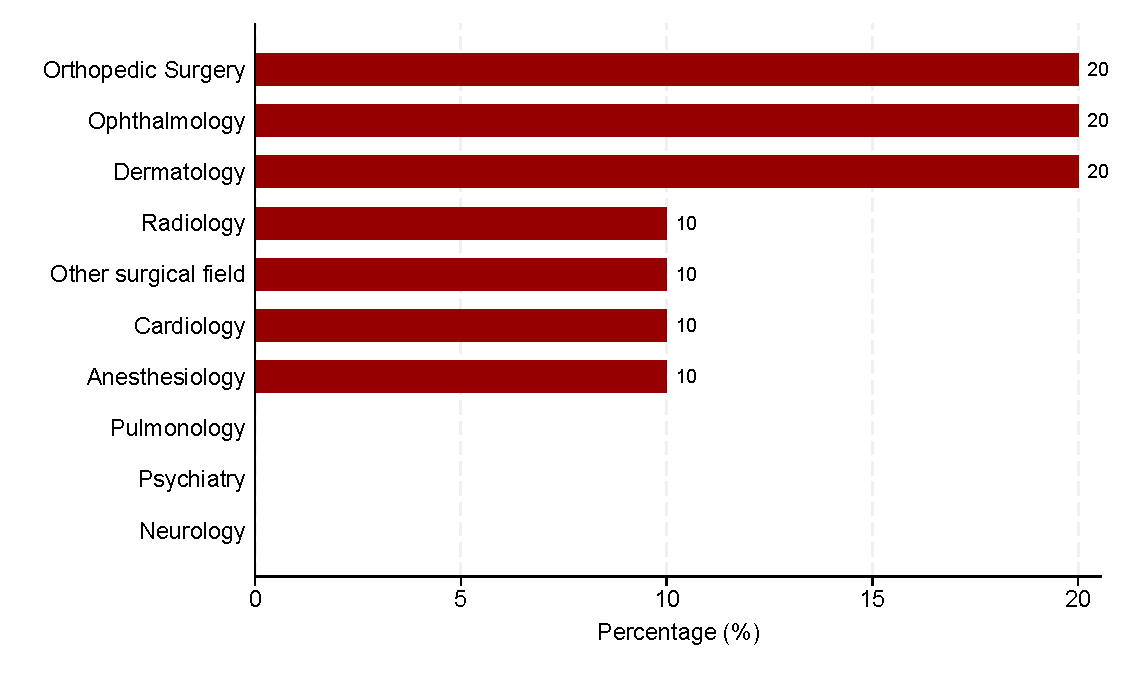
\includegraphics[width=1\linewidth]{Pre-Survey/figures/fin_motive_top_share_PC.pdf}
\end{adjustbox}
    \end{subfigure}
            \begin{subfigure}{0.45\textwidth}
        \caption{Bottom 5}
    \begin{adjustbox}{width=1\linewidth}  
    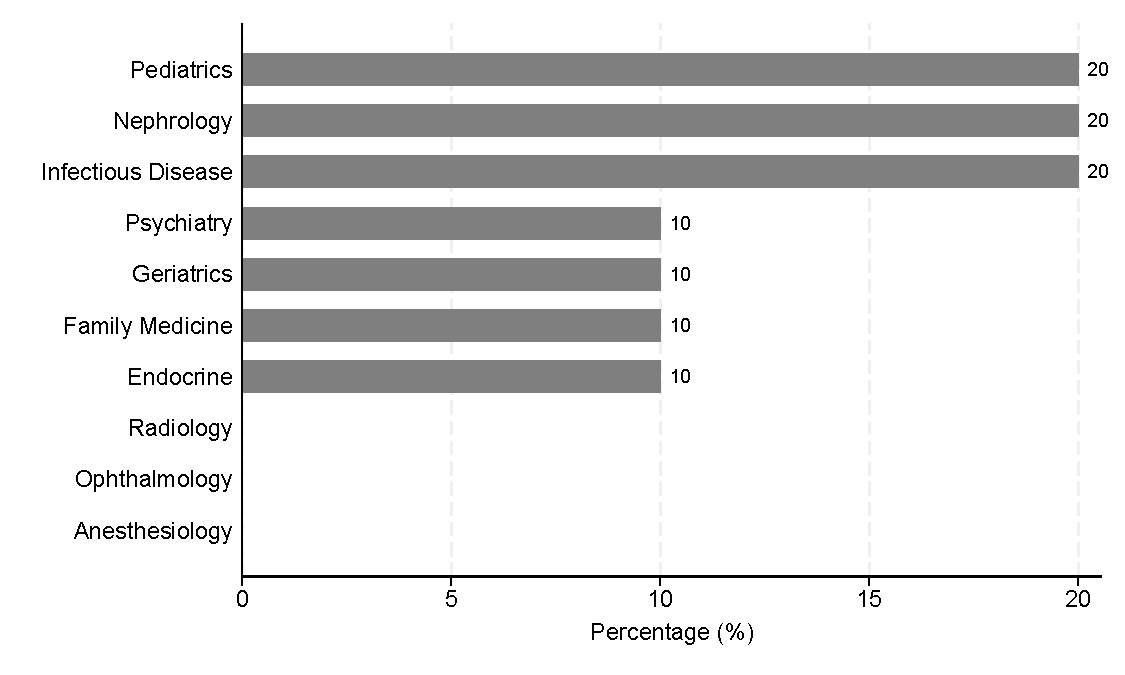
\includegraphics[width=1\linewidth]{Pre-Survey/figures/fin_motive_bottom_share_PC.pdf}
\end{adjustbox}
    \end{subfigure}
    \label{fig:top_bottom_pc}
     {\parbox{\linewidth}{           %notes
		\scriptsize{{{ \textit{Notes:} Notes: The figure displays the medical specialties cited by primary care physicians as most (Top 5) and least (Bottom 5) financially motivated. Percentages represent the share of all selections within each category (Top 5 or Bottom 5). Respondents could select up to five specialties per category. Panel (a) reports the five specialties with the largest Top-5 shares; Panel (b) reports the five with the largest Bottom-5 shares}}}}}
\end{figure}

\begin{figure}[H]
    \centering
    \caption{Among Specialists: Categorization of Medical Specialties by Financial Motivation }
 \begin{subfigure}{0.45\textwidth}
        \caption{Top 5}
    \begin{adjustbox}{width=1\linewidth}  
    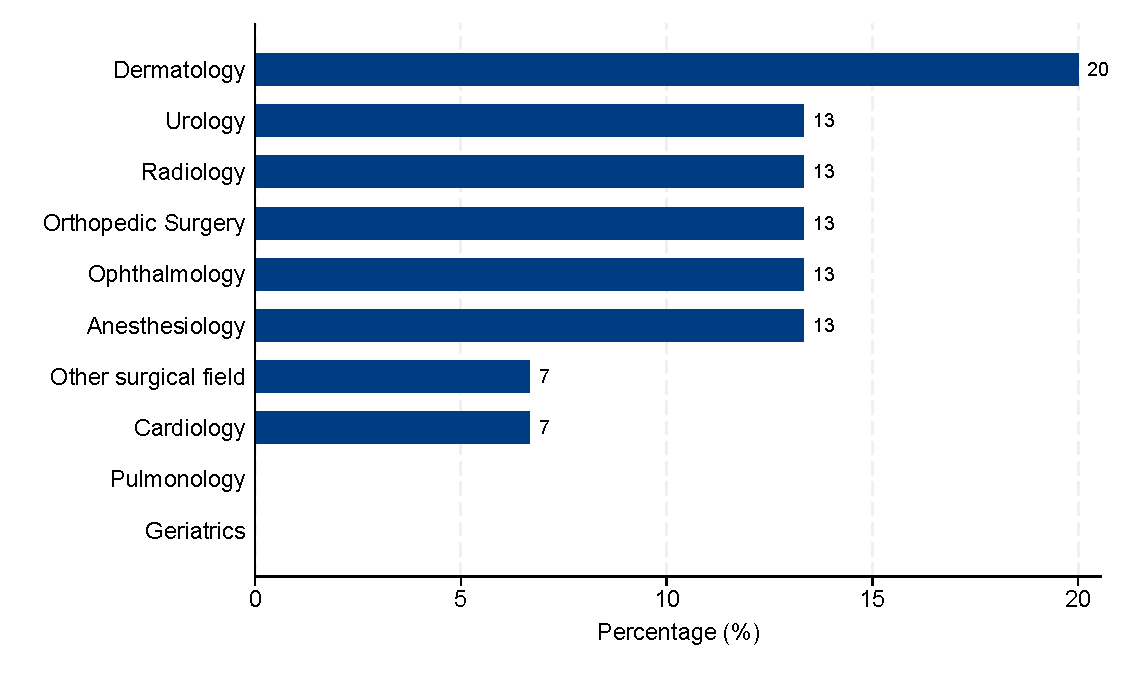
\includegraphics[width=1\linewidth]{Pre-Survey/figures/fin_motive_top_share_SP.pdf}
\end{adjustbox}
    \end{subfigure}
            \begin{subfigure}{0.45\textwidth}
        \caption{Bottom 5}
    \begin{adjustbox}{width=1\linewidth}  
    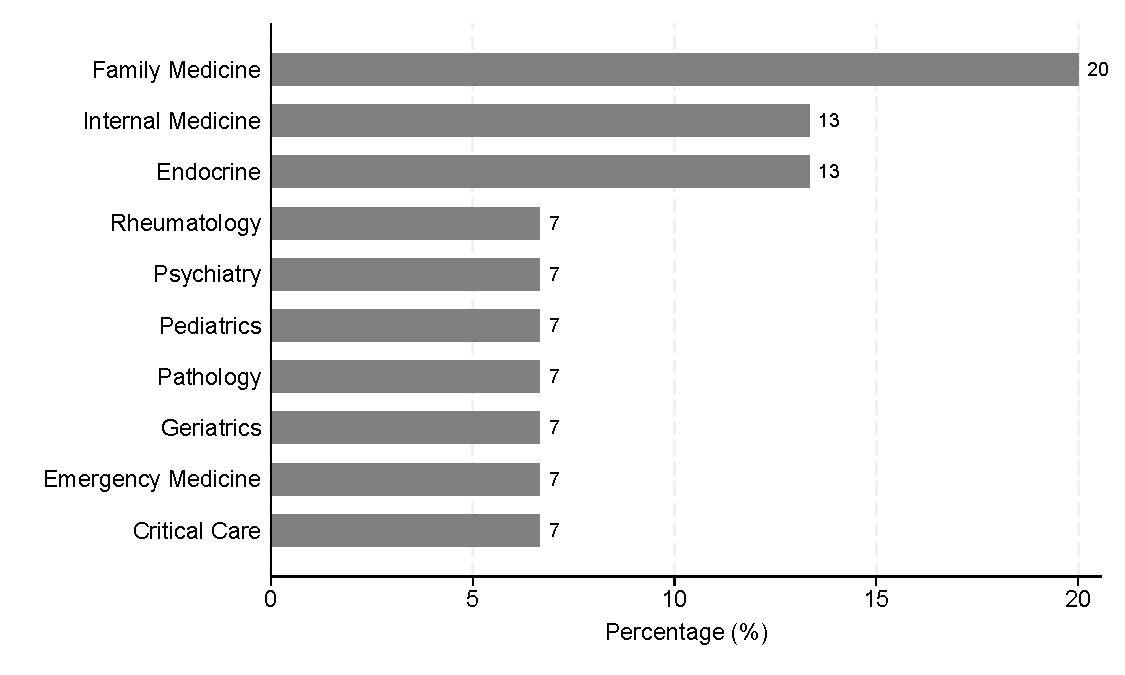
\includegraphics[width=1\linewidth]{Pre-Survey/figures/fin_motive_bottom_share_SP.pdf}
\end{adjustbox}
    \end{subfigure}
    \label{fig:top_bottom_sp}
     {\parbox{\linewidth}{           %notes
		\scriptsize{{{ \textit{Notes:} Notes: The figure displays the medical specialties cited by specialists as most (Top 5) and least (Bottom 5) financially motivated. Percentages represent the share of all selections within each category (Top 5 or Bottom 5) and therefore sum to 100\% within each panel. Respondents could select up to five specialties per category. Panel (a) reports the five specialties with the largest Top-5 shares; Panel (b) reports the five with the largest Bottom-5 shares}}}}}
\end{figure}

\section{Categorization of Belief Questions} 

\begin{table}[H]
    \centering
    \caption{Categorization of Belief Questions}
        \begin{adjustbox}{width=0.95\linewidth} 
\begin{tabular}{lcccccccc}\toprule
 & \multicolumn{4}{c}{Among Primary Care Physicians} & \multicolumn{4}{c}{Among Specialists} \\
\cmidrule(lr){2-5} \cmidrule(lr){6-9}
Medical field & \% Physician benefits  & \% Patient benefits & \% Both & \% Neither & \% Physician benefits  & \% Patient benefits & \% Both & \% Neither \\ \midrule
Union improves pay & 100 & 0 & 0 & 0 & 67 & 0 & 0 & 33 \\
Union improves benefits & 100 & 0 & 0 & 0 & 67 & 0 & 0 & 33 \\
Union reduces overwork & 50 & 0 & 50 & 0 & 33 & 0 & 67 & 0 \\
\midrule
Union improves patient care & 0 & 0 & 100 & 0 & 0 & 33 & 33 & 33 \\
Union improves autonomy & 50 & 0 & 50 & 0 & 0 & 33 & 33 & 33 \\
Union improves staffing & 0 & 0 & 100 & 0 & 0 & 0 & 67 & 33 \\
\midrule
Union reduces burnout & 0 & 0 & 100 & 0 & 33 & 0 & 33 & 33 \\
\bottomrule\end{tabular}

\end{adjustbox}
     \parbox{\linewidth}{
        	\vspace{.2cm}
        		\scriptsize{\scriptsize{{\emph{Notes}: The table displays statistics for the overall sample of physicians. "Total" shows the number of observations used to calculate each percentage, and "Percentages (\%)" indicates the percentage of respondents in each group.}}}}
    \label{tab:ai_table}
\end{table}

%\begin{figure}[H]
%	\centering
%	\caption{Categorization of Belief Questions}
%	\label{fig:cat_belief}
%	\begin{adjustbox}{max width=\textwidth}
%		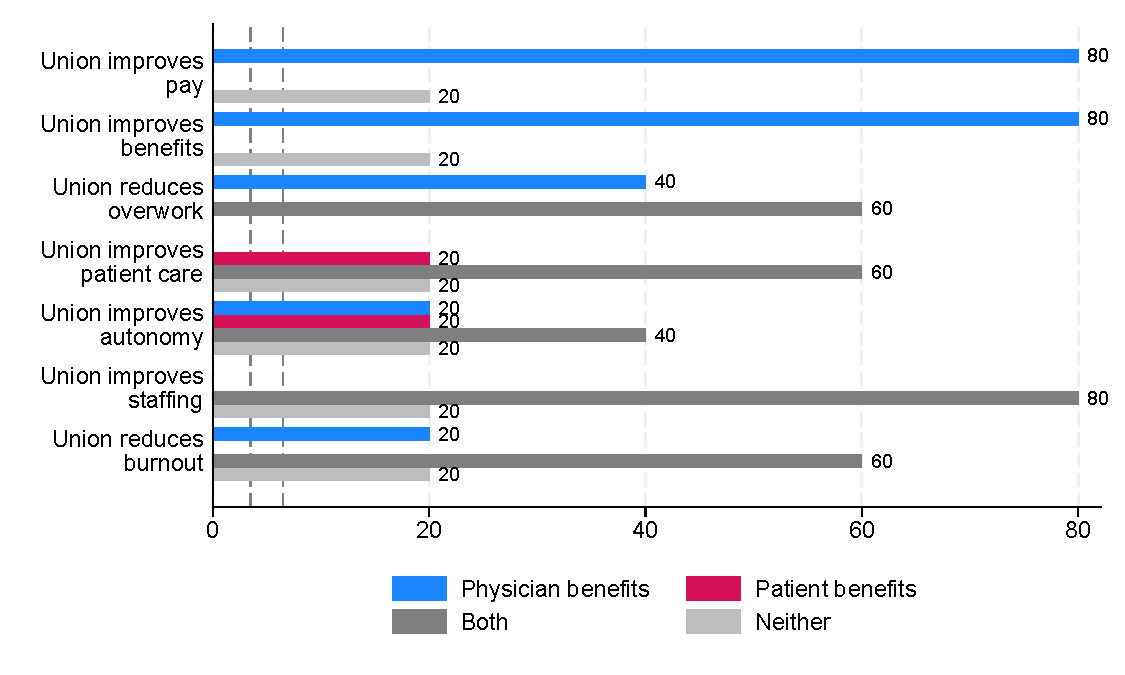
\includegraphics{Pre-Survey/figures/cat_statements_outtype.pdf}
%	\end{adjustbox}
%	\parbox{.9\linewidth}{
%		\vspace{.2cm}
%		\scriptsize{\emph{Notes}: The figure displays the categorization of belief statements about unionization across four categories: personal physician benefits, patient benefits, cannot categorize, and other. Percentages represent the share of total categorizations for each statement, and values across categories for a given statement sum to 100\%.}
%	}
%\end{figure}

\begin{figure}[H]
    \centering
    \caption{Categorization of Belief Questions by Physician Type}
       \begin{subfigure}{0.8\textwidth}
        \caption{Among Primary Care Physicians}
    \begin{adjustbox}{width=1\linewidth}  
    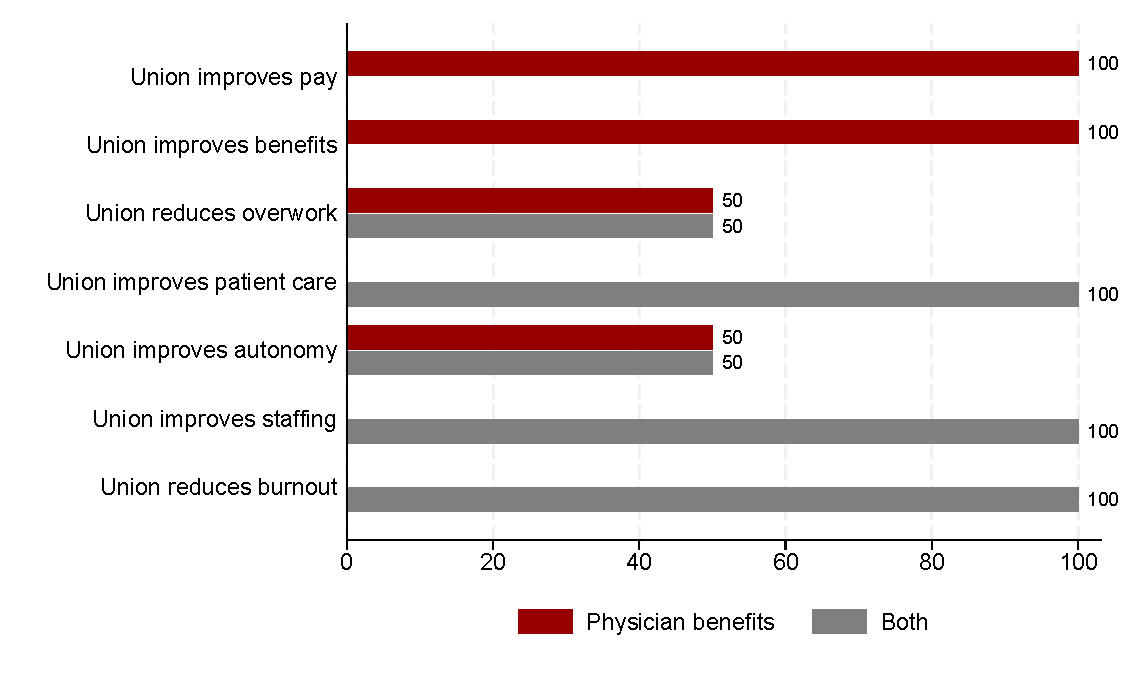
\includegraphics[width=1\linewidth]{Pre-Survey/figures/cat_statements_outtype_PC.pdf}
\end{adjustbox}
    \end{subfigure}
    \\
        \begin{subfigure}{0.8\textwidth}
        \caption{Among Specialists}
    \begin{adjustbox}{width=1\linewidth}  
    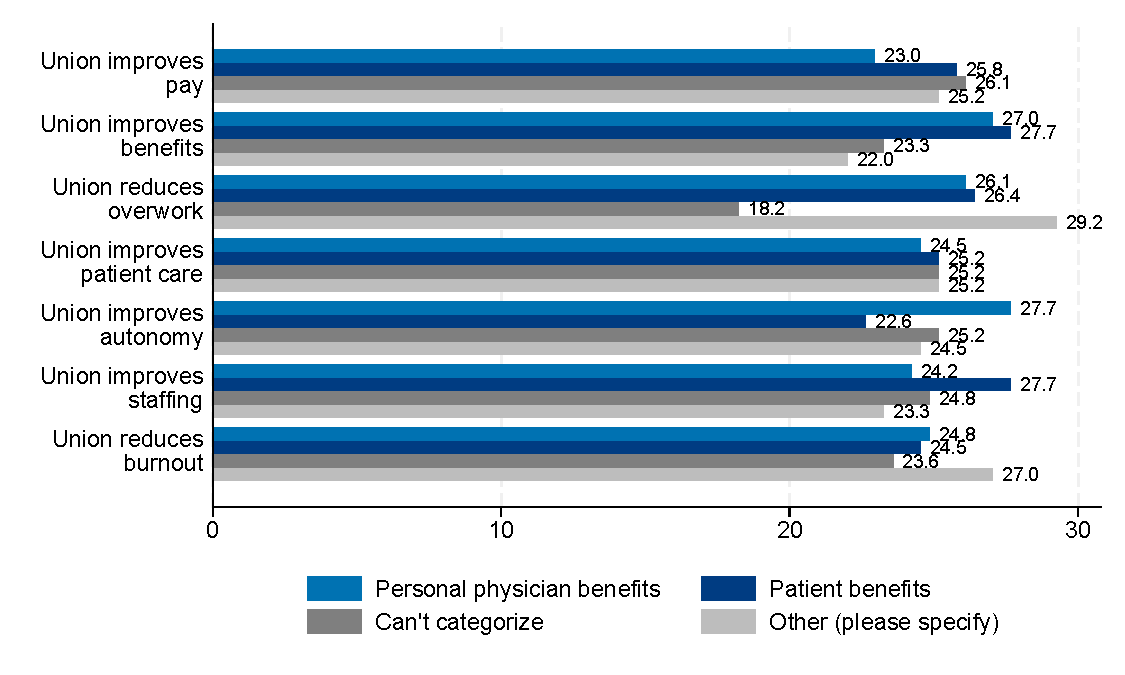
\includegraphics[width=1\linewidth]{Pre-Survey/figures/cat_statements_outtype_SP.pdf}
\end{adjustbox}
    \end{subfigure}
    \label{fig:distributed}
     {\parbox{\linewidth}{           %notes
		\scriptsize{{{ \textit{Notes:} The figure displays the categorization of belief statements about unionization across four categories: personal physician benefits, patient benefits, cannot categorize, and other. Percentages represent the share of total categorizations for each statement, and values across categories for a given statement sum to 100\%. Panel (a) and Panel (b) show the plots for primary care physicians and specialists, respectively.}}}}}
\end{figure}

\clearpage

\section{Views on Physicians' Unionization} 

\begin{table}[H]
    \centering
    \caption{Views on Physicians' Unionization}
        \begin{adjustbox}{width=1\linewidth} 
\begin{tabular}{lcccccc} \toprule & \multicolumn{2}{c}{\textbf{Primary Care}} & \multicolumn{2}{c}{\textbf{Specialists}} & \multicolumn{1}{c}{\textbf{All}} \\ \cmidrule(lr){2-3} \cmidrule(lr){4-5} \cmidrule(lr){6-7} & Total  & Percentage (\%) & Total  & Percentage (\%) & Total  & Percentage (\%)
                &\multicolumn{2}{c}{}&\multicolumn{2}{c}{}&\multicolumn{2}{c}{}\\
\midrule
\emph{Views on physician's unions}&         &         &         &         &         &         \\
Would join union&       29&       41&      318&       42&      347&       41\\
Would recommend medicine if physicians unionized&       29&       52&      318&       42&      347&       42\\
Would stay if physicians unionized&       29&       45&      318&       41&      347&       41\\
\vspace{0.1em} \\ \emph{Views on physician's unions - open text}&         &         &         &         &         &         \\
Would join union (text observed)&       29&      100&      318&      100&      347&      100\\
Would recommend medicine if physicians unionized (text observed)&       29&      100&      318&      100&      347&      100\\
Would stay if physicians unionized (text observed)&       29&      100&      318&      100&      347&      100\\
\vspace{0.1em} \\ \emph{Willingness to stay}&         &         &         &         &         &         \\
Want to stay 3 more years&       29&       52&      318&       40&      347&       41\\
Would stay if offered job elsewhere&       29&       28&      318&       41&      347&       40\\
\bottomrule \end{tabular}

\end{adjustbox}
     \parbox{\linewidth}{
        	\vspace{.2cm}
        		\scriptsize{\scriptsize{{\emph{Notes}: The table displays statistics for the overall sample of physicians. "Total" shows the number of observations used to calculate each percentage, and "Percentages (\%)" indicates the percentage of respondents in each group. }}}}
    \label{tab:ai_table}
\end{table}

\begin{figure}[H]
	\centering
	\caption{Views on Physicians' Unionization}
	\label{fig:cat_belief}
	\begin{adjustbox}{width=0.85\textwidth}
		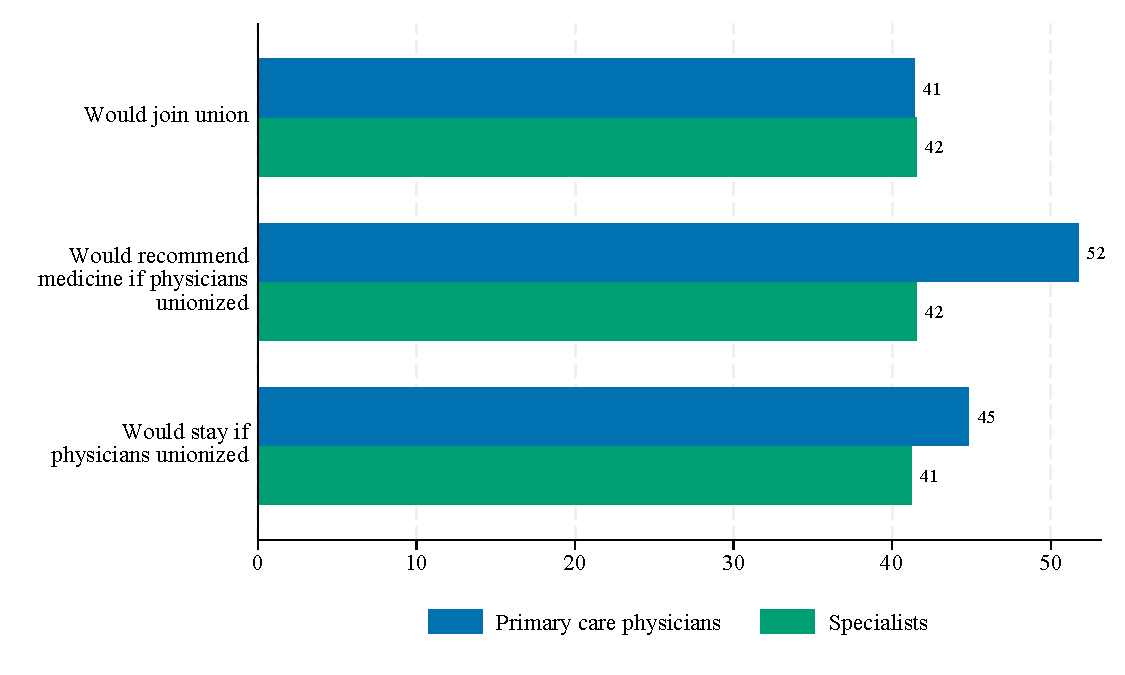
\includegraphics{Pre-Survey/figures/sec_stage_byphystype.pdf}
	\end{adjustbox}
	\parbox{.9\linewidth}{
		\vspace{.2cm}
		\scriptsize{\emph{Notes}: The figure reports the share of primary care physicians and specialists who agreed with each statement.}
	}
\end{figure}


\clearpage

\section{Real Stakes}

\begin{table}[H]
    \centering
    \caption{Real Stakes}
        \begin{adjustbox}{width=0.75\linewidth} 
\begin{tabular}{lcccccc} \toprule & \multicolumn{2}{c}{\textbf{Primary Care}} & \multicolumn{2}{c}{\textbf{Specialists}} & \multicolumn{1}{c}{\textbf{All}} \\ \cmidrule(lr){2-3} \cmidrule(lr){4-5} \cmidrule(lr){6-7} & Total  & Percentage (\%) & Total  & Percentage (\%) & Total  & Percentage (\%)
                &\multicolumn{2}{c}{}&\multicolumn{2}{c}{}&\multicolumn{2}{c}{}\\
\midrule
Wants info on unions (non-unionized only)&      347&       52&       29&       55&      318&       52\\
\vspace{0.1em} \\ \emph{Support petition}&         &         &         &         &         &         \\
Instruction understanding (ama)&       10&       80&        1&      100&        9&       78\\
Instruction understanding (ama and society)&      337&       48&       28&       46&      309&       48\\
RECODE of petition\_support\_ama (petition\_support\_ama)&       10&       70&        1&      100&        9&       67\\
RECODE of petition\_support\_spe (petition\_support\_spe)&      337&       48&       28&       43&      309&       49\\
\bottomrule \end{tabular}

\end{adjustbox}
     \parbox{\linewidth}{
        	\vspace{.2cm}
        		\scriptsize{\scriptsize{{\emph{Notes}:The table displays statistics for the overall sample of physicians. "Total" shows the number of observations used to calculate each percentage, and "Percentages (\%)" indicates the percentage of respondents in each group.}}}}
    \label{tab:stakes_table}
\end{table}

\clearpage

\section{Feedback}

\begin{table}[H]
    \centering
    \caption{Feedback}
        \begin{adjustbox}{width=0.45\linewidth}  
\begin{tabular}{l*{1}{cc}}
\toprule
                &    Total&Percentage (\%)\\
\midrule
\vspace{0.1em} \\ \emph{Feedback on the survey}&         &         \\
Feedback on the survey (observed)&        5&       80\\
Survey confusing sections/questions&        5&        0\\
\vspace{0.1em} \\ \emph{Purpose of the survey}&         &         \\
Purpose of the survey (observed)&        5&      100\\
\vspace{0.1em} \\ \emph{Perceived survey bias}&         &         \\
Survey felt left-biased&        5&       20\\
Survey felt right-biased&        5&        0\\
Survey felt unbiased&        5&       80\\
\vspace{0.1em} \\ \emph{Additional comments}&         &         \\
Additional comments (observed)&        5&       80\\
\bottomrule
\end{tabular}

\end{adjustbox}
     \parbox{\linewidth}{
        	\vspace{.2cm}
        		\scriptsize{\scriptsize{{\emph{Notes}: The table displays statistics for the overall sample of physicians. "Total" shows the number of observations used to calculate each percentage, and "Percentages (\%)" indicates the percentage of respondents in each group.}}}}
    \label{tab:ai_table}
\end{table}

\clearpage

\section{Open text} 

\subsection{Categorization of belief questions}


    \begin{itemize}
        \item \href{https://www.dropbox.com/scl/fi/x5nio65ohv7o42dk6sc4i/feedback_belief_questions.csv?rlkey=cxxseve65x52cfwgaqtiqsoqa&dl=0}{Do you have any feedback on these questions?}
        \item \href{https://www.dropbox.com/scl/fi/unuuezlgufxpxlz3sxysk/open_text_other_beliefs.csv?rlkey=lioi0nr74mga9ylyxm0fjhlbk&dl=0}{Please list up to three additional changes you anticipate a physicians’ union could bring to your workplace that were not mentioned above. Start with the one you consider most important.}
    \end{itemize}

\subsection{Views on Physician Unionization}

    \begin{itemize}
        \item \href{https://www.dropbox.com/scl/fi/7l946s8rsn3pz3ay3ngr9/open_text_union_join.csv?rlkey=qoo5pf8flkn84kworsynjg04s&dl=0}{Open text: To what extent do you agree or disagree with the following statement ``If there was a physicians’ union at my workplace, I would join it.''}
        \item \href{https://www.dropbox.com/scl/fi/n2hpphm5tddg6sma346gd/open_text_union_rec_prob.csv?rlkey=oykwwwy15xkis5lvbs8k2egbh&dl=0}{Open text: To what extent do you agree or disagree with the following statement ``I would be more likely to recommend a career in medicine if physicians were unionized.''}
        \item \href{https://www.dropbox.com/scl/fi/fencs6zg509nr4s1vi2mf/open_text_union_plans.csv?rlkey=96ore8pdjvjsphxajimymd0ae&dl=0}{Open text: To what extent do you agree or disagree with the following statement ``I would be more likely to stay in my current job if physicians were unionized.''}
    \end{itemize}

    
\subsection{Survey Feedback}

    \begin{itemize}
        \item \href{https://www.dropbox.com/scl/fi/sygw2qcnhu6lxjr7p7cl8/open_text_survey_feedback.csv?rlkey=gwzrqoluii5eecgb56vm52jp5&dl=0}{Do you have any feedback on this survey?}
        \item \href{https://www.dropbox.com/scl/fi/63m9mx1qkhc6r95838idl/open_text_survey_purpose.csv?rlkey=03ila2825gpvtx0q3lhb406pd&dl=0}{Please provide us with your impression of the survey’s purpose.}
        \item \href{https://www.dropbox.com/scl/fi/ekae24vyahmeddiydrsh6/open_text_confusing_questions.csv?rlkey=fr8oiwpg6ww70cpkrt44fimnt&dl=0}{For responders who replied ``Yes'': Did you find any part or question in the survey unclear or confusing? }
        \href{https://www.dropbox.com/scl/fi/jzzi5srfjrdm8gzk779j8/open_text_add_comments.csv?rlkey=sa5sgk8u70xxtxd4n65bc3sjz&dl=0}{Anything else you would like to share?}
    \end{itemize}

    \clearpage
\appendix

\section{Appendix}

\subsection{Contact List Currently Available}

\begin{table}[H]
    \centering
    \caption{Distribution of Physician Specialties by Provider Type (REDI Data, N = 99,488)}
    	\begin{adjustbox}{max width=0.8\textwidth}
\begin{tabular}{lrrrrrrr} \toprule & \multicolumn{2}{c}{\textbf{Primary Care}} & \multicolumn{2}{c}{\textbf{Specialists}} & \multicolumn{2}{c}{\textbf{ER}} & \multicolumn{1}{c}{\textbf{All}} \\ \cmidrule(lr){2-3} \cmidrule(lr){4-5} \cmidrule(lr){6-7} & Total  & Percentage (\%) & Total  & Percentage (\%) & Total  & Percentage (\%) & Total \\ & \multicolumn{1}{r}{(1)} & \multicolumn{1}{r}{(2)} & \multicolumn{1}{r}{(3)} & \multicolumn{1}{r}{(4)} & \multicolumn{1}{r}{(5)}
                    &\multicolumn{1}{c}{}&\multicolumn{1}{c}{}&\multicolumn{1}{c}{}&\multicolumn{1}{c}{}&\multicolumn{1}{c}{}&\multicolumn{1}{c}{}&\multicolumn{1}{c}{}\\
\hline
Allergy and immunology&           0&           0&         598&           1&           0&           0&         598\\
Anesthesiology      &           0&           0&        5881&          12&           0&           0&        5881\\
Cardiology          &           0&           0&        3780&           8&           0&           0&        3780\\
Dermatology         &           0&           0&        1682&           3&           0&           0&        1682\\
Emergency medical services&         123&           0&           0&           0&           0&           0&         123\\
Emergency medicine  &           0&           0&           0&           0&        7641&         100&        7641\\
Endocrinology, diabetes and metabolism&           0&           0&        1040&           2&           0&           0&        1040\\
Family medicine     &       15929&          38&           0&           0&           0&           0&       15929\\
General practice    &         275&           1&           0&           0&           0&           0&         275\\
Geriatrics          &           0&           0&         986&           2&           0&           0&         986\\
Internal medicine   &       17248&          41&        8538&          17&           0&           0&       25786\\
Medical genetics    &           0&           0&          99&           0&           0&           0&          99\\
Neurological surgery&           0&           0&         799&           2&           0&           0&         799\\
Neurology           &           0&           0&        2528&           5&           0&           0&        2528\\
Oncology (cancer)   &           0&           0&        3100&           6&           0&           0&        3100\\
Ophthalmology       &           0&           0&        2388&           5&           0&           0&        2388\\
Orthopedics         &           0&           0&        3414&           7&           0&           0&        3414\\
Otolaryngology      &           0&           0&        1306&           3&           0&           0&        1306\\
Pathology           &           0&           0&        1305&           3&           0&           0&        1305\\
Pediatrics          &        8528&          20&           0&           0&           0&           0&        8528\\
Plastic surgery     &           0&           0&         913&           2&           0&           0&         913\\
Radiology           &           0&           0&        4701&           9&           0&           0&        4701\\
Surgery             &           0&           0&        5394&          11&           0&           0&        5394\\
Urology             &           0&           0&        1292&           3&           0&           0&        1292\\
\midrule Observations & & 42103 & & 49744 & & 7641 & 99488 \\ \bottomrule \end{tabular}

\end{adjustbox}
     \parbox{.9\linewidth}{
        	\vspace{.2cm}
        		\scriptsize{\scriptsize{{\emph{Notes}: The table presents statistics for primary care physicians, specialists, ER, and the full sample. “Share (\%)” indicates the proportion of respondents in each specialty, while “Total” shows the corresponding number of physicians.}}}}
    \label{tab:spec_table}
\end{table}

\subsection{Sanity Checks on Random Sampling}\label{sanity}

\begin{table}[H]
    \centering
    \caption{Population and Sample Shares of Primary Care Physicians and Specialists by Medical Field}
              \begin{adjustbox}{width=0.85\linewidth}  
\begin{tabular}{lrrrrrrrr} \toprule & \multicolumn{4}{c}{\textbf{Primary Care}} & \multicolumn{4}{c}{\textbf{Specialists}} \\ \cmidrule(lr){2-5} \cmidrule(lr){6-9} & \multicolumn{2}{c}{\textbf{REDI-data}} & \multicolumn{2}{c}{\textbf{Sample}} & \multicolumn{2}{c}{\textbf{REDI-data}} & \multicolumn{2}{c}{\textbf{Sample}} \\ \cmidrule(lr){2-3} \cmidrule(lr){4-5} \cmidrule(lr){6-7} \cmidrule(lr){8-9} & Total & Percentage (\%) & Total & Percentage (\%) & Total & Percentage (\%) & Total & Percentage (\%)
            &\multicolumn{1}{c}{}&\multicolumn{1}{c}{}&\multicolumn{1}{c}{}&\multicolumn{1}{c}{}&\multicolumn{1}{c}{}&\multicolumn{1}{c}{}&\multicolumn{1}{c}{}&\multicolumn{1}{c}{}\\
\hline
Allergy and immunology&           0&           0&           0&           0&         598&           1&          17&           2\\
Anesthesiology&           0&           0&           0&           0&        5881&          12&         115&          12\\
Cardiology  &           0&           0&           0&           0&        3780&           8&          72&           7\\
Dermatology &           0&           0&           0&           0&        1682&           3&          29&           3\\
Emergency medical services&         123&           0&           3&           0&           0&           0&           0&           0\\
Endocrinology, diabetes and metabolism&           0&           0&           0&           0&        1040&           2&          22&           2\\
Family medicine&       15929&          38&         356&          36&           0&           0&           0&           0\\
General practice&         275&           1&          10&           1&           0&           0&           0&           0\\
Geriatrics  &           0&           0&           0&           0&         986&           2&          13&           1\\
Internal medicine&       17248&          41&         419&          42&        8538&          17&         157&          16\\
Medical genetics&           0&           0&           0&           0&          99&           0&           2&           0\\
Neurological surgery&           0&           0&           0&           0&         799&           2&          17&           2\\
Neurology   &           0&           0&           0&           0&        2528&           5&          53&           5\\
Oncology (cancer)&           0&           0&           0&           0&        3100&           6&          63&           6\\
Ophthalmology&           0&           0&           0&           0&        2388&           5&          49&           5\\
Orthopedics &           0&           0&           0&           0&        3414&           7&          76&           8\\
Otolaryngology&           0&           0&           0&           0&        1306&           3&          29&           3\\
Pathology   &           0&           0&           0&           0&        1305&           3&          18&           2\\
Pediatrics  &        8528&          20&         212&          21&           0&           0&           0&           0\\
Plastic surgery&           0&           0&           0&           0&         913&           2&          13&           1\\
Radiology   &           0&           0&           0&           0&        4701&           9&         109&          11\\
Surgery     &           0&           0&           0&           0&        5394&          11&         114&          11\\
Urology     &           0&           0&           0&           0&        1292&           3&          32&           3\\
\midrule Observations & 42103 & & 1000 & & 49744 & & 1000 & \\ \bottomrule \end{tabular}

\end{adjustbox}
     \parbox{.9\linewidth}{
        	\vspace{.2cm}
        		\scriptsize{\scriptsize{{\emph{Notes}: The table shows statistics for the population and the random sample for each group: primary care physicians and specialists. "Share (\%)" indicates the percentage of respondents in each group, and "Total" shows the number of observations used to calculate each percentage.}}}}
    \label{tab:sanity_spec}
\end{table}

\begin{table}[H]
    \centering
    \caption{Population and Sample Shares of Primary Care Physicians and Specialists by Region}
              \begin{adjustbox}{width=0.65\linewidth}  
\begin{tabular}{lrrrrrrrr} \toprule & \multicolumn{4}{c}{\textbf{Primary Care}} & \multicolumn{4}{c}{\textbf{Specialists}} \\ \cmidrule(lr){2-5} \cmidrule(lr){6-9} & \multicolumn{2}{c}{\textbf{REDI-data}} & \multicolumn{2}{c}{\textbf{Sample}} & \multicolumn{2}{c}{\textbf{REDI-data}} & \multicolumn{2}{c}{\textbf{Sample}} \\ \cmidrule(lr){2-3} \cmidrule(lr){4-5} \cmidrule(lr){6-7} \cmidrule(lr){8-9} & Total & Percentage (\%) & Total & Percentage (\%) & Total & Percentage (\%) & Total & Percentage (\%)
            &\multicolumn{1}{c}{}&\multicolumn{1}{c}{}&\multicolumn{1}{c}{}&\multicolumn{1}{c}{}&\multicolumn{1}{c}{}&\multicolumn{1}{c}{}&\multicolumn{1}{c}{}&\multicolumn{1}{c}{}\\
\hline
Midwest     &        8432&          20&         192&          19&       12558&          25&         261&          26\\
Northeast   &       10452&          25&         233&          23&       10466&          21&         201&          20\\
South       &       13621&          32&         327&          33&       18385&          37&         363&          36\\
West        &        9598&          23&         248&          25&        8335&          17&         175&          18\\
\midrule Observations & 42103 & & 1000 & & 49744 & & 1000 & \\ \bottomrule \end{tabular}

\end{adjustbox}
     \parbox{.9\linewidth}{
        	\vspace{.2cm}
        		\scriptsize{\scriptsize{{\emph{Notes}: The table shows statistics for the population and the random sample for each group: primary care physicians and specialists. "Share (\%)" indicates the percentage of respondents in each group, and "Total" shows the number of observations used to calculate each percentage.}}}}
    \label{tab:sanity_geo}
\end{table}



%\singlespace
%\bibliography{biblio}

\end{document}

\section{Results for ER}

\subsection{Demographics}

\begin{table}[H]
    \centering
    \caption{Summary Statistics for Demographics of ER Doctors}
              \begin{adjustbox}{width=0.55\linewidth}  
\begin{tabular}{l*{1}{cc}}
\toprule
                &Percentage (\%)&    Total\\
\midrule
\emph{Place of birth}&         &         \\
Born in U.S.    &       80&        5\\
\vspace{0.1em} \\ \emph{Age group}&         &         \\
Age <25         &        0&        5\\
Age 25–34       &       20&        5\\
Age 35–44       &       20&        5\\
Age 45–54       &       60&        5\\
Age 55–64       &        0&        5\\
Age 65+         &        0&        5\\
\vspace{0.1em} \\ \emph{Sex}&         &         \\
Male            &       40&        5\\
Female          &       60&        5\\
Other gender    &        0&        5\\
\vspace{0.1em} \\ \emph{Marital status}&         &         \\
Single          &        0&        5\\
Married         &      100&        5\\
Separated       &        0&        5\\
Widowed         &        0&        5\\
\vspace{0.1em} \\ \emph{Ethnicity}&         &         \\
Hispanic        &        0&        5\\
\vspace{0.1em} \\ \emph{Race}&         &         \\
White           &       60&        5\\
Black           &        0&        5\\
Native American &        0&        5\\
Pacific Islander&        0&        5\\
Asian           &       40&        5\\
Other race      &        0&        5\\
Mixed race      &        0&        5\\
\vspace{0.1em} \\ \emph{Political affiliation}&         &         \\
Republican      &       20&        5\\
Democrat        &       40&        5\\
Independent     &       40&        5\\
Other party     &        0&        5\\
Physician union at current workplace&       20&        5\\
Work ZIP (observed)&      100&        5\\
\bottomrule
\end{tabular}

\end{adjustbox}
     \parbox{.9\linewidth}{
        	\vspace{.2cm}
        		\scriptsize{\scriptsize{{\emph{Notes}: The table displays statistics for the overall sample of physicians. "Share (\%)" indicates the percentage of respondents in each group, and "Total" shows the number of observations used to calculate each percentage.}}}}
    \label{tab:demo_table}
\end{table}

\subsection{Categorization of Medical Fields among ER doctors}

\begin{table}[H]
    \centering
    \caption{Among ER Doctors: Categorization of Medical Field by Physician Types}
    \begin{adjustbox}{width=0.75\linewidth} 
    \begin{tabular}{lccccccc}\toprule 
    & \multicolumn{2}{c}{Primary Care Physician} & \multicolumn{2}{c}{Specialist} & \multicolumn{2}{c}{Difficult to classify} & {All groups} \\
    \cmidrule(lr){2-3} \cmidrule(lr){4-5} \cmidrule(lr){6-7}  
    {Medical field}&{Total}&{Percentage (\%)}&{Total}&{Percentage (\%)}&{Total}&{Percentage (\%)} &{Percentage (\%)} \tabularnewline
\midrule
Anesthesiology&1&25&0&0&3&75&100 \tabularnewline
Cardiology&1&33&1&33&1&33&100 \tabularnewline
Allergy and Immunology&0&0&2&67&1&33&100 \tabularnewline
Ophthalmology&1&17&2&33&3&50&100 \tabularnewline
Orthopedic Surgery&2&67&1&33&0&0&100 \tabularnewline
Pathology&2&40&0&0&3&60&100 \tabularnewline
Pediatrics&0&0&9&56&7&44&100 \tabularnewline
Radiology&2&40&0&0&3&60&100 \tabularnewline
General Surgery&1&33&1&33&1&33&100 \tabularnewline
Urology&2&100&0&0&0&0&100 \tabularnewline
Dermatology&2&25&1&12&5&62&100 \tabularnewline
Endocrine&2&50&0&0&2&50&100 \tabularnewline
Geriatrics&2&29&3&43&2&29&100 \tabularnewline
Internal Medicine&6&38&3&19&7&44&100 \tabularnewline
Emergency Medicine&4&25&7&44&5&31&100 \tabularnewline
Family Medicine&7&44&4&25&5&31&100 \tabularnewline
Neurology&1&50&1&50&0&0&100 \tabularnewline
Hematology/Oncology&0&&0&&0&&0 \tabularnewline
Critical Care&1&50&0&0&1&50&100 \tabularnewline
Gastroenterology and Hepatology&1&33&0&0&2&67&100 \tabularnewline
Infectious Disease&2&50&1&25&1&25&100 \tabularnewline
Nephrology&4&57&1&14&2&29&100 \tabularnewline
Obstetrics and Gynecology&2&40&1&20&2&40&100 \tabularnewline
Other surgical field (e.g., Neurosurgery, Plastic Surgery, ENT/Otolaryngology)&2&67&0&0&1&33&100 \tabularnewline
Other medical field (e.g., Sleep Medicine, Sports Medicine, Medical Genetics)&1&50&1&50&0&0&100 \tabularnewline
Psychiatry&1&33&2&67&0&0&100 \tabularnewline
Pulmonology&2&33&2&33&2&33&100 \tabularnewline
Rheumatology&1&50&1&50&0&0&100 \tabularnewline
Transplant&1&25&0&0&3&75&100 \tabularnewline
\bottomrule 

    \end{tabular}
    \end{adjustbox}
    \label{tab:med_field_cat_phystype}
          {\parbox{1\linewidth}{           %notes
    		\scriptsize{{{ \textit{Notes:} The table displays statistics for the sample of ER doctors. "Total" shows the number of observations used to calculate each percentage, and "Percentages (\%)" indicates the percentage of respondents in each group. Percentages are calculated row-wise, so values across columns for a given medical field sum to 100\%.}}}}}
\end{table}

\subsection{Categorization of Medical Fields by Financial Motivation among ER Doctors}

\begin{table}[H]
    \centering
    \caption{Categorization of Medical Specialties by Financial Motivation (Top 5 vs. Bottom 5)}
    \begin{adjustbox}{width=0.55\linewidth} 
    \begin{tabular}{lcccc}\toprule & \multicolumn{2}{c}{Top 5} & \multicolumn{2}{c}{Bottom 5} \\ \cmidrule(lr){2-3} \cmidrule(lr){4-5} 
    {Specialty}&{Total}&{Percentage (\%)}&{Total}&{Percentage (\%)} \tabularnewline
\midrule \addlinespace[\belowrulesep]
Allergy and Immunology&3&4&5&6 \tabularnewline
Anesthesiology&3&4&2&2 \tabularnewline
Cardiology&2&2&7&9 \tabularnewline
Dermatology&2&2&0&0 \tabularnewline
Endocrine&1&1&2&2 \tabularnewline
Geriatrics&2&2&0&0 \tabularnewline
Emergency Medicine&2&2&2&2 \tabularnewline
Family Medicine&3&4&4&5 \tabularnewline
Internal Medicine&3&4&6&8 \tabularnewline
Neurology&2&2&4&5 \tabularnewline
Hematology/Oncology&3&4&2&2 \tabularnewline
Ophthalmology&3&4&1&1 \tabularnewline
Orthopedic Surgery&4&5&3&4 \tabularnewline
Pathology&2&2&2&2 \tabularnewline
Pediatrics&2&2&2&2 \tabularnewline
Radiology&3&4&2&2 \tabularnewline
General Surgery&3&4&1&1 \tabularnewline
Urology&5&6&1&1 \tabularnewline
Critical Care&2&2&6&8 \tabularnewline
Gastroenterology and Hepatology&2&2&5&6 \tabularnewline
Infectious Disease&4&5&4&5 \tabularnewline
Nephrology&3&4&1&1 \tabularnewline
Obstetrics and Gynecology&1&1&2&2 \tabularnewline
Other medical field (e.g., Sleep Medicine, Sports Medicine, Medical Genetics)&3&4&4&5 \tabularnewline
Other surgical field (e.g., Neurosurgery, Plastic Surgery, ENT/Otolaryngology)&2&2&3&4 \tabularnewline
Psychiatry&4&5&2&2 \tabularnewline
Pulmonology&2&2&1&1 \tabularnewline
Rheumatology&4&5&4&5 \tabularnewline
Transplant&5&6&2&2 \tabularnewline
Total&80&&80& \tabularnewline
\bottomrule 


    \end{tabular}
    \end{adjustbox}
    \label{tab:med_field_cat_finmov}
          {\parbox{1\linewidth}{           %notes
		\scriptsize{{{ \textit{Notes:} The table reports the distribution of medical specialties ranked among the top 5 and bottom 5 fields in terms of financial motivation. “Total” indicates the number of times each specialty was placed in the respective category across all respondents. “Percentage (\%)” shows the share of these placements relative to the total number of top (or bottom) 5 selections. Percentages within each column sum to 100\%.}}}}}
\end{table}


\subsection{Categorization of Belief Questions} 

\begin{table}[H]
    \centering
    \caption{Categorization of Belief Questions}
        \begin{adjustbox}{width=0.95\linewidth} 
    \begin{tabular}{lcccccccc}\toprule & \multicolumn{2}{c}{Personal Physician benefits} & \multicolumn{2}{c}{Patient benefits} & \multicolumn{2}{c}{Can't categorize} & \multicolumn{2}{c}{Other (please specify)} \\ \cmidrule(lr){2-3} \cmidrule(lr){4-5} \cmidrule(lr){6-7} \cmidrule(lr){8-9} 
{Statement}&{Total}&{Percentage (\%)}&{Total}&{Percentage (\%)}&{Total}&{Percentage (\%)}&{Total}&{Percentage (\%)} \tabularnewline
\midrule \addlinespace[\belowrulesep]
Union improves pay&1&6&4&25&5&31&6&38 \tabularnewline
Union improves benefits&6&38&3&19&2&12&5&31 \tabularnewline
Union reduces overwork&5&31&4&25&4&25&3&19 \tabularnewline
Union improves patient care&1&6&6&38&7&44&2&12 \tabularnewline
Union improves autonomy&4&25&4&25&7&44&1&6 \tabularnewline
Union improves staffing&2&12&3&19&5&31&6&38 \tabularnewline
Union reduces burnout&4&25&6&38&3&19&3&19 \tabularnewline
\bottomrule 
    \end{tabular}
\end{adjustbox}
     \parbox{\linewidth}{
        	\vspace{.2cm}
        		\scriptsize{\scriptsize{{\emph{Notes}: The table displays statistics for the sample of ER doctors. "Total" shows the number of observations used to calculate each percentage, and "Percentages (\%)" indicates the percentage of respondents in each group.}}}}
    \label{tab:ai_table}
\end{table}

\begin{figure}[H]
	\centering
	\caption{Categorization of Belief Questions}
	\label{fig:cat_belief}
	\begin{adjustbox}{max width=\textwidth}
		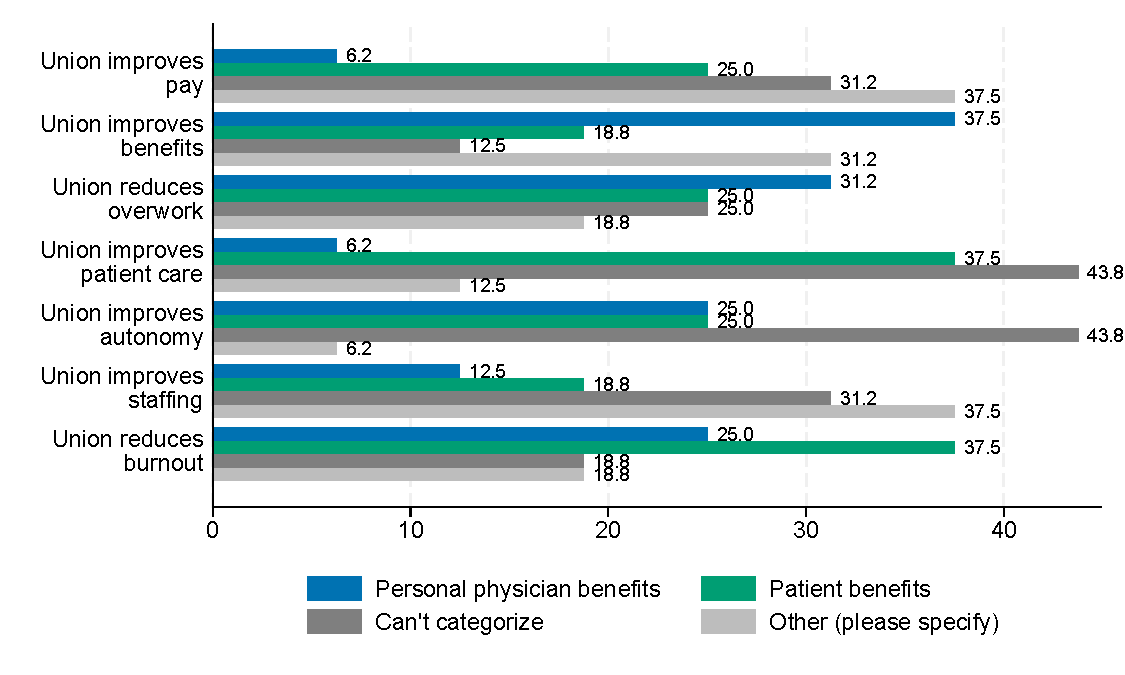
\includegraphics{Pre-Survey/figures/cat_statements_outtype_ER.pdf}
	\end{adjustbox}
	\parbox{.9\linewidth}{
		\vspace{.2cm}
		\scriptsize{\emph{Notes}: The figure displays the categorization of belief statements about unionization across four categories: personal physician benefits, patient benefits, cannot categorize, and other. Percentages represent the share of total categorizations for each statement, and values across categories for a given statement sum to 100\%.}
	}
\end{figure}



\subsection{Views on Physicians' Unionization} 

\begin{table}[H]
    \centering
    \caption{Views on Physicians' Unionization}
        \begin{adjustbox}{width=1\linewidth} 
\begin{tabular}{lcc} \toprule & \multicolumn{2}{c}{\textbf{ER Physicians}} \\ \cmidrule(lr){2-3} & Total  & Percentage (\%)
                &\multicolumn{2}{c}{}\\
\midrule
\emph{Views on physician's unions}&         &         \\
Would join union&       16&       38\\
Would recommend medicine if physicians unionized&       16&       75\\
Would stay if physicians unionized&       16&       31\\
\vspace{0.1em} \\ \emph{Views on physician's unions - open text}&         &         \\
Would join union (text observed)&       16&      100\\
Would recommend medicine if physicians unionized (text observed)&       16&      100\\
Would stay if physicians unionized (text observed)&       16&      100\\
\vspace{0.1em} \\ \emph{Willingness to stay}&         &         \\
Want to stay 3 more years&       16&       44\\
Would stay if offered job elsewhere&       16&       31\\
\bottomrule \end{tabular}

\end{adjustbox}
     \parbox{\linewidth}{
        	\vspace{.2cm}
        		\scriptsize{\scriptsize{{\emph{Notes}: The table displays statistics for the sample of ER doctors. "Total" shows the number of observations used to calculate each percentage, and "Percentages (\%)" indicates the percentage of respondents in each group. }}}}
    \label{tab:ai_table}
\end{table}

\begin{figure}[H]
	\centering
	\caption{Views on Physicians' Unionization}
	\label{fig:cat_belief}
	\begin{adjustbox}{width=0.85\textwidth}
		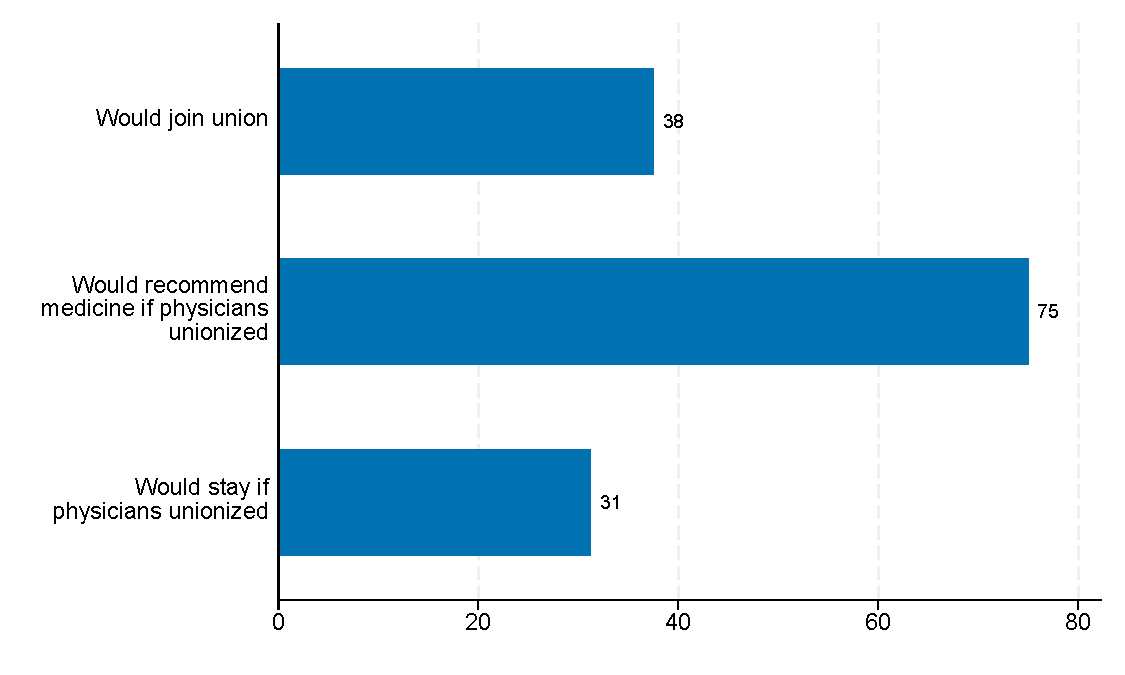
\includegraphics{Pre-Survey/figures/sec_stage_byphystype_ER.pdf}
	\end{adjustbox}
	\parbox{.7\linewidth}{
		\vspace{.2cm}
		\scriptsize{\emph{Notes}: The figure reports the share of ER doctors who agreed with each statement.}
	}
\end{figure}




\begin{comment}    
\begin{table}[H]
    \centering
    \caption{COVID-19 Block Before Treatment}
\input{Phys_main_survey/tables_updated/covid_byphystype_1}
     \parbox{\linewidth}{
        	\vspace{.2cm}
        		\scriptsize{\scriptsize{{\emph{Notes}: The table displays statistics for PC-ER physicians, PC-No ER physicians, specialists, and the overall sample.}}}}
    \label{tab:ai_table}
\end{table}

\begin{table}[H]
    \centering
    \caption{COVID-19 Block After Treatment}
\input{Phys_main_survey/tables_updated/covid_byphystype_0}
     \parbox{\linewidth}{
        	\vspace{.2cm}
        		\scriptsize{\scriptsize{{\emph{Notes}: The table displays statistics for PC-ER physicians, PC-No ER physicians, specialists, and the overall sample.}}}}
    \label{tab:ai_table}
\end{table}
\end{comment}
